
\section{Software Design}

With regards to our project, we shall consider our simulation as software for the SDS. Hence, this subsection explains the overall design of the simulation system including a UML class diagram.

This particular system is structured around three core modules: \textbf{Environment}, \textbf{Perception}, and \textbf{Locomotion}. These modules interact to allow for teleoperating the robot with posture adaptation on rough terrain. 

Figure \ref{fig:uml_class_diagram} shows the UML class diagram.

\begin{figure}[h!]
    \centering
    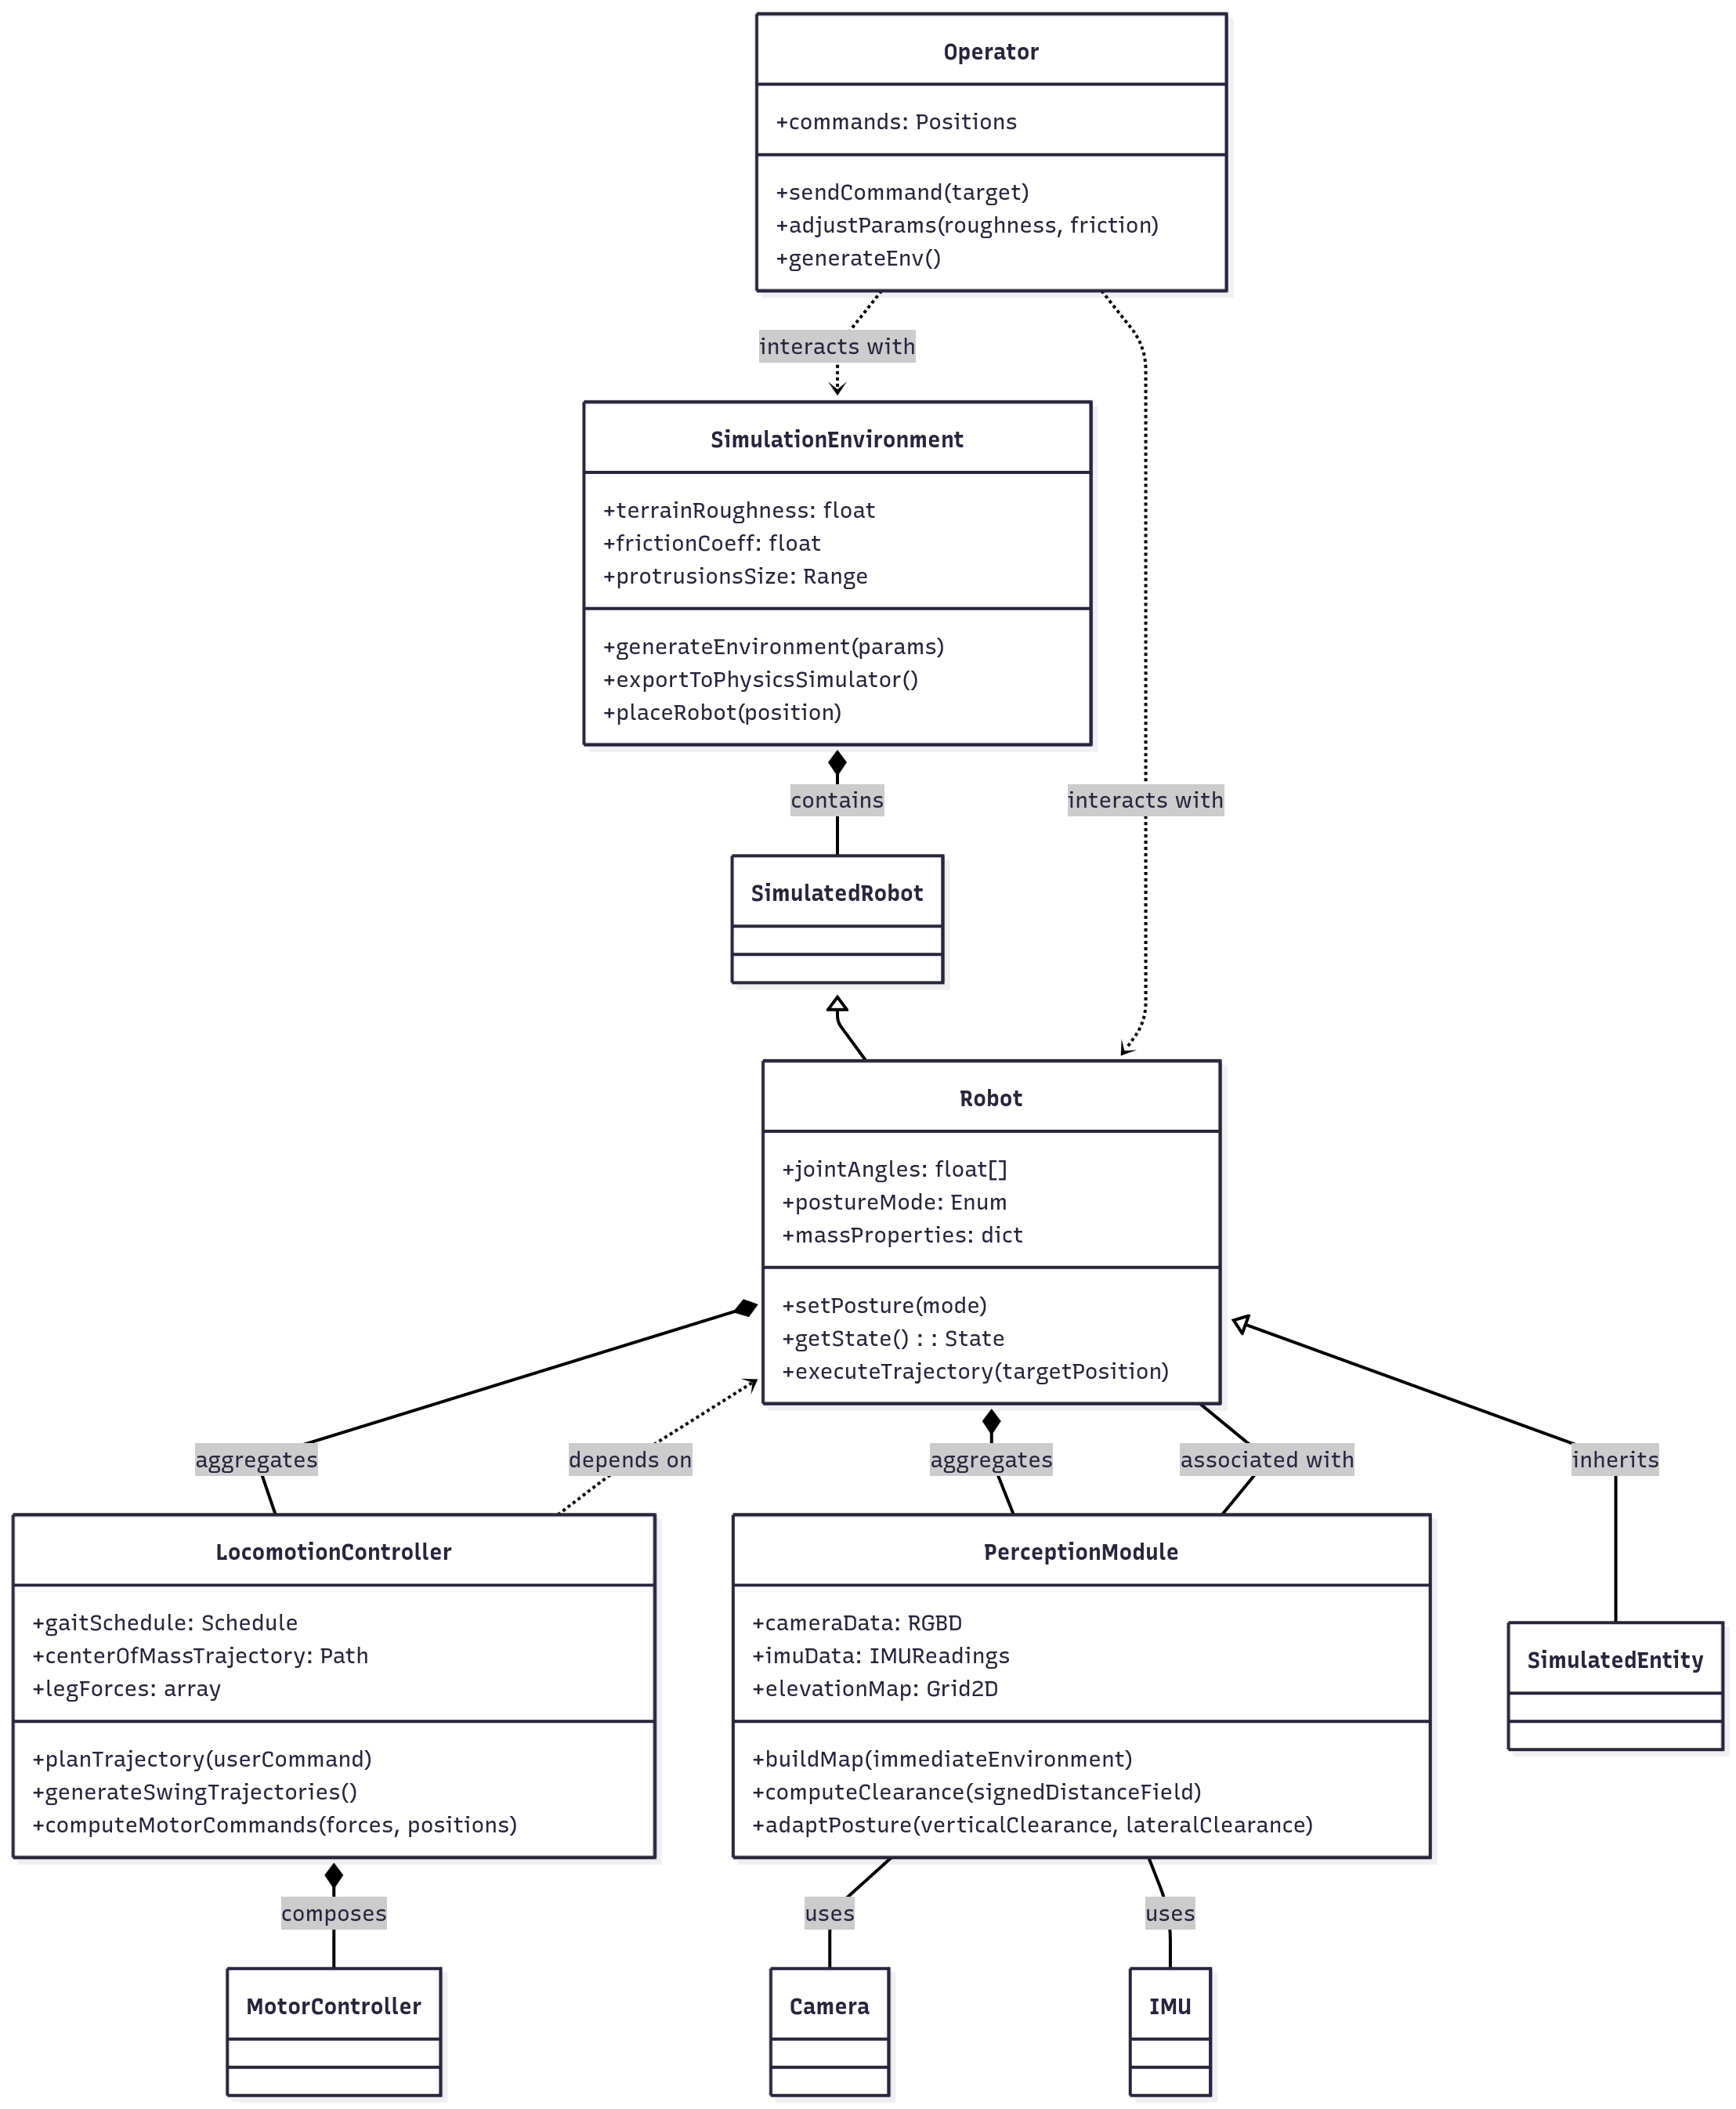
\includegraphics[width=0.85\textwidth]{full.png}
    \caption{Class Diagram for the Legged Robot System.}
    \label{fig:uml_class_diagram}
\end{figure}

The Operator acts as the user interface where the user teleoperates the robot. They also have the liberty to adjust the parameters of the environment such as terrain roughness and friction. The SimulationEnvironment is where the testing happens. It is reliant on the mentioned parameters and generates the environment to show to the physics simulator (Gazebo). Then, the SimulatedRobot is placed within the scene. The Robot is the T-Hex in simulation and manages state information while executing commanded trajectories. It aggregates both the LocomotionController and PerceptionModule; the former manages gaits and trajectories through Ground Reaction Forces for legs in stance and smooth swing leg trajectories to send to the MotorController which executes the commands, and the latter is where the robot senses data from the environment via RGB-D andIMU readings to construct the elevation map. This map is used to calculate clearance; that is, collision-free space; through a signed distance field. This is used to adapt the robot's posture based on the vertical and lateral clearance.

\section{Data Design}

While we do not need persistent data and hence a database, it is worth discussing data structures used in the project. All data is managed within simulation and Docker environment. This data flows through Figures \ref{fig:locomotion_diagram} and \ref{fig:perception_diagram}, and the hardware data path in a physical build is shown in Figure \ref{fig:hardware_diagram}.

The most important data structure is the Elevation Map. It is a 2D grid entity timestamped for accuracy meant to store terrain heights. From here is derived the Signed Distance Field (SDF) which models clearance by retrieving distance values to obstacles. 

The robot's behavioral data relies on Posture Parameters, a structure defining modes using attributes
namely leg spread, fixed body height, etc. On the other hand, the environment relies on Simulation Parameter which are roughness, friction range, maximum protrusion size (6cm), etc. For brevity's sake, we shall not be including the kinematic and DRL diagrams here.

\begin{figure}[h!]
    \centering
    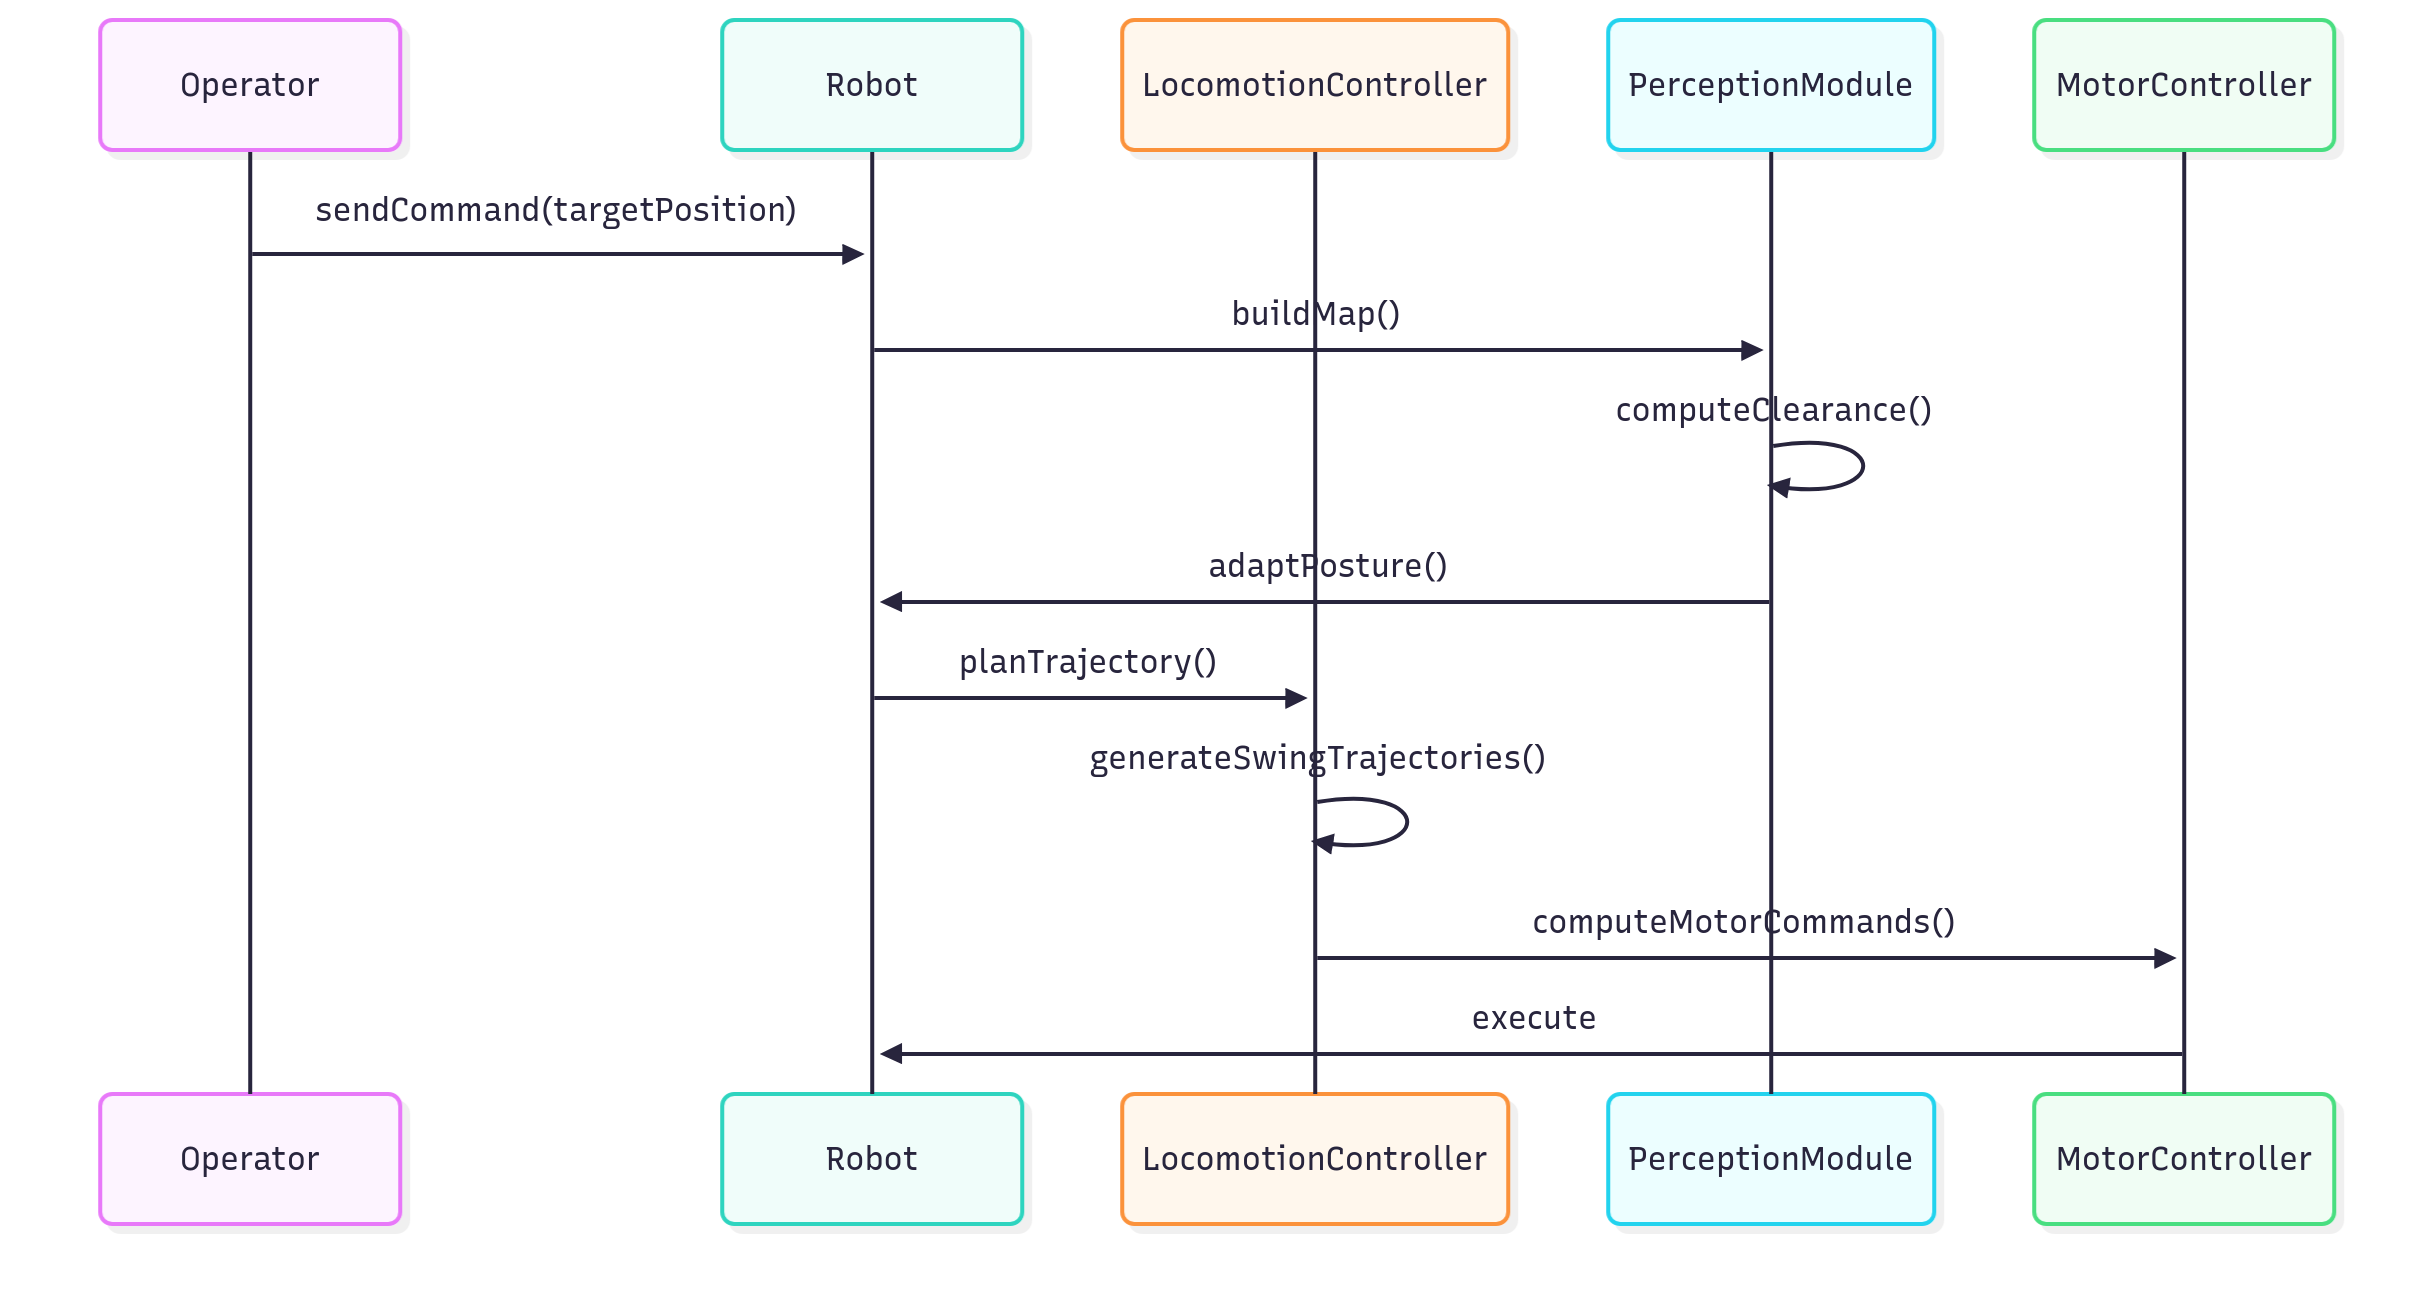
\includegraphics[width=1.0\textwidth]{locomotion.png}
    \caption{Sequence Diagram for the Locomotion Pipeline, detailing the interaction between the operator, robot, and core control modules.}
    \label{fig:locomotion_diagram}
\end{figure}

\begin{figure}[h!]
    \centering
    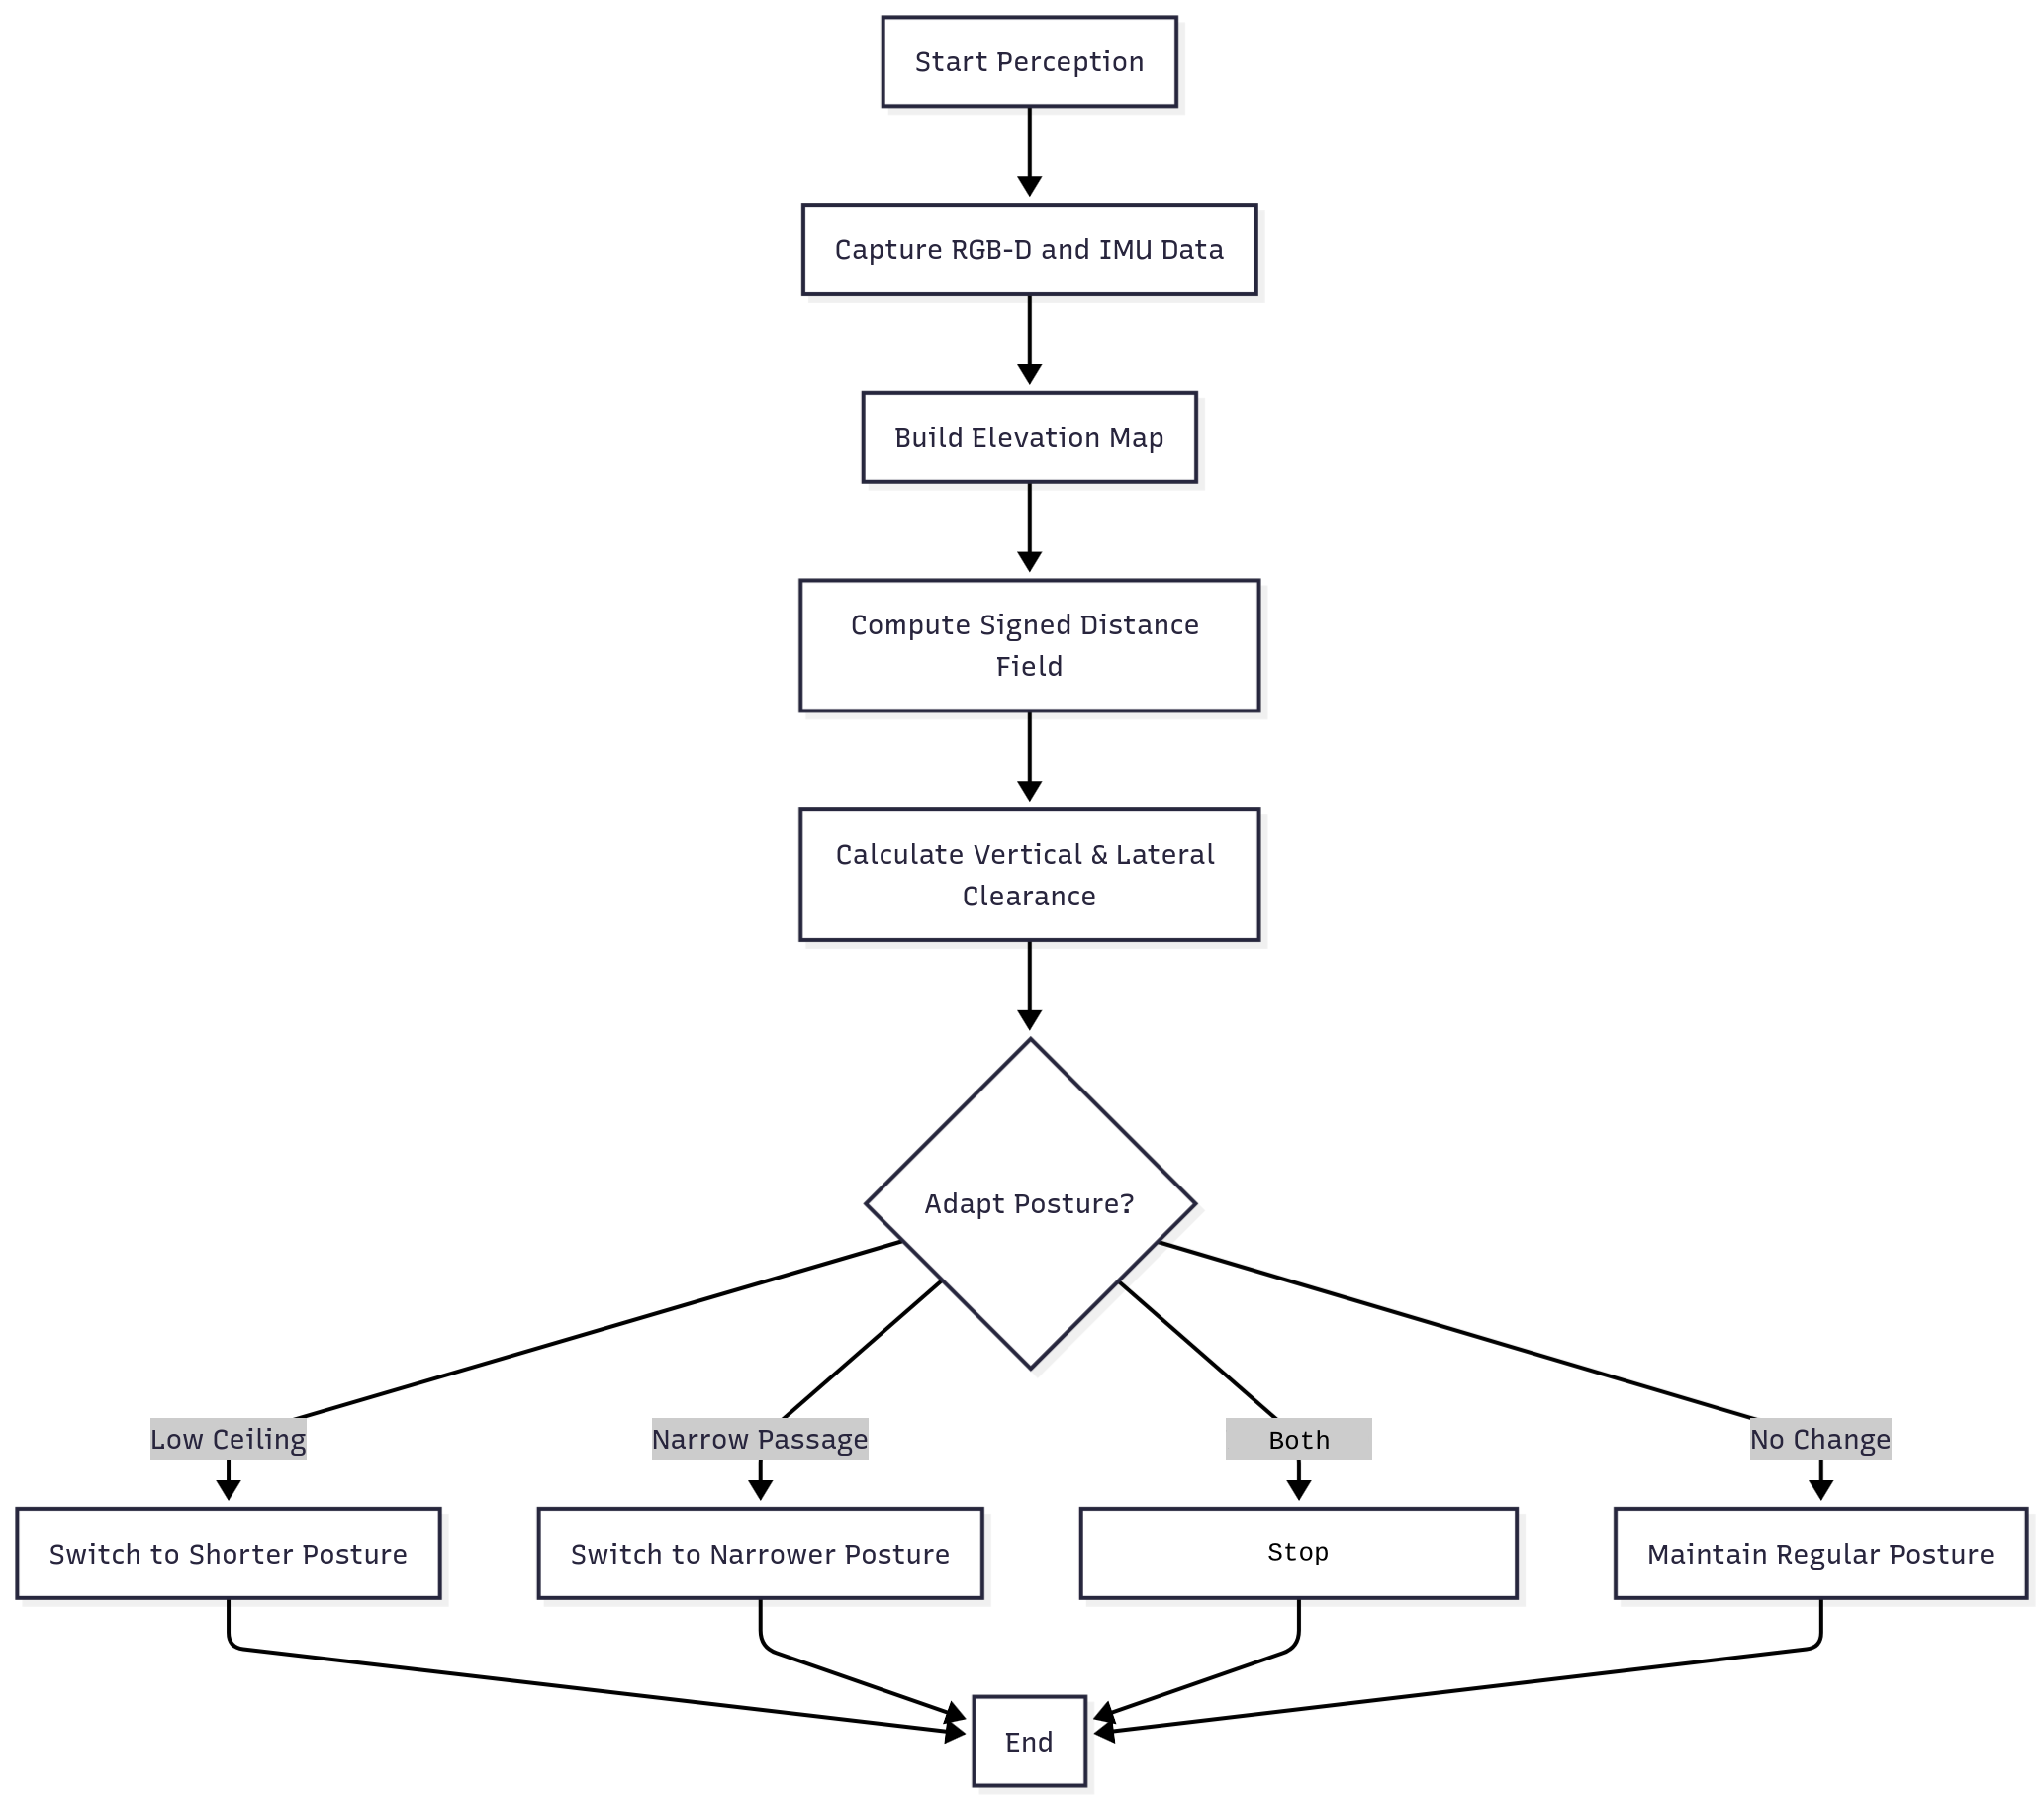
\includegraphics[width=0.8\textwidth]{perception.png}
    \caption{Flowchart for the Perception Pipeline, illustrating the steps from data capture to posture adaptation decision.}
    \label{fig:perception_diagram}
\end{figure}

\begin{figure}[h!]
    \centering
    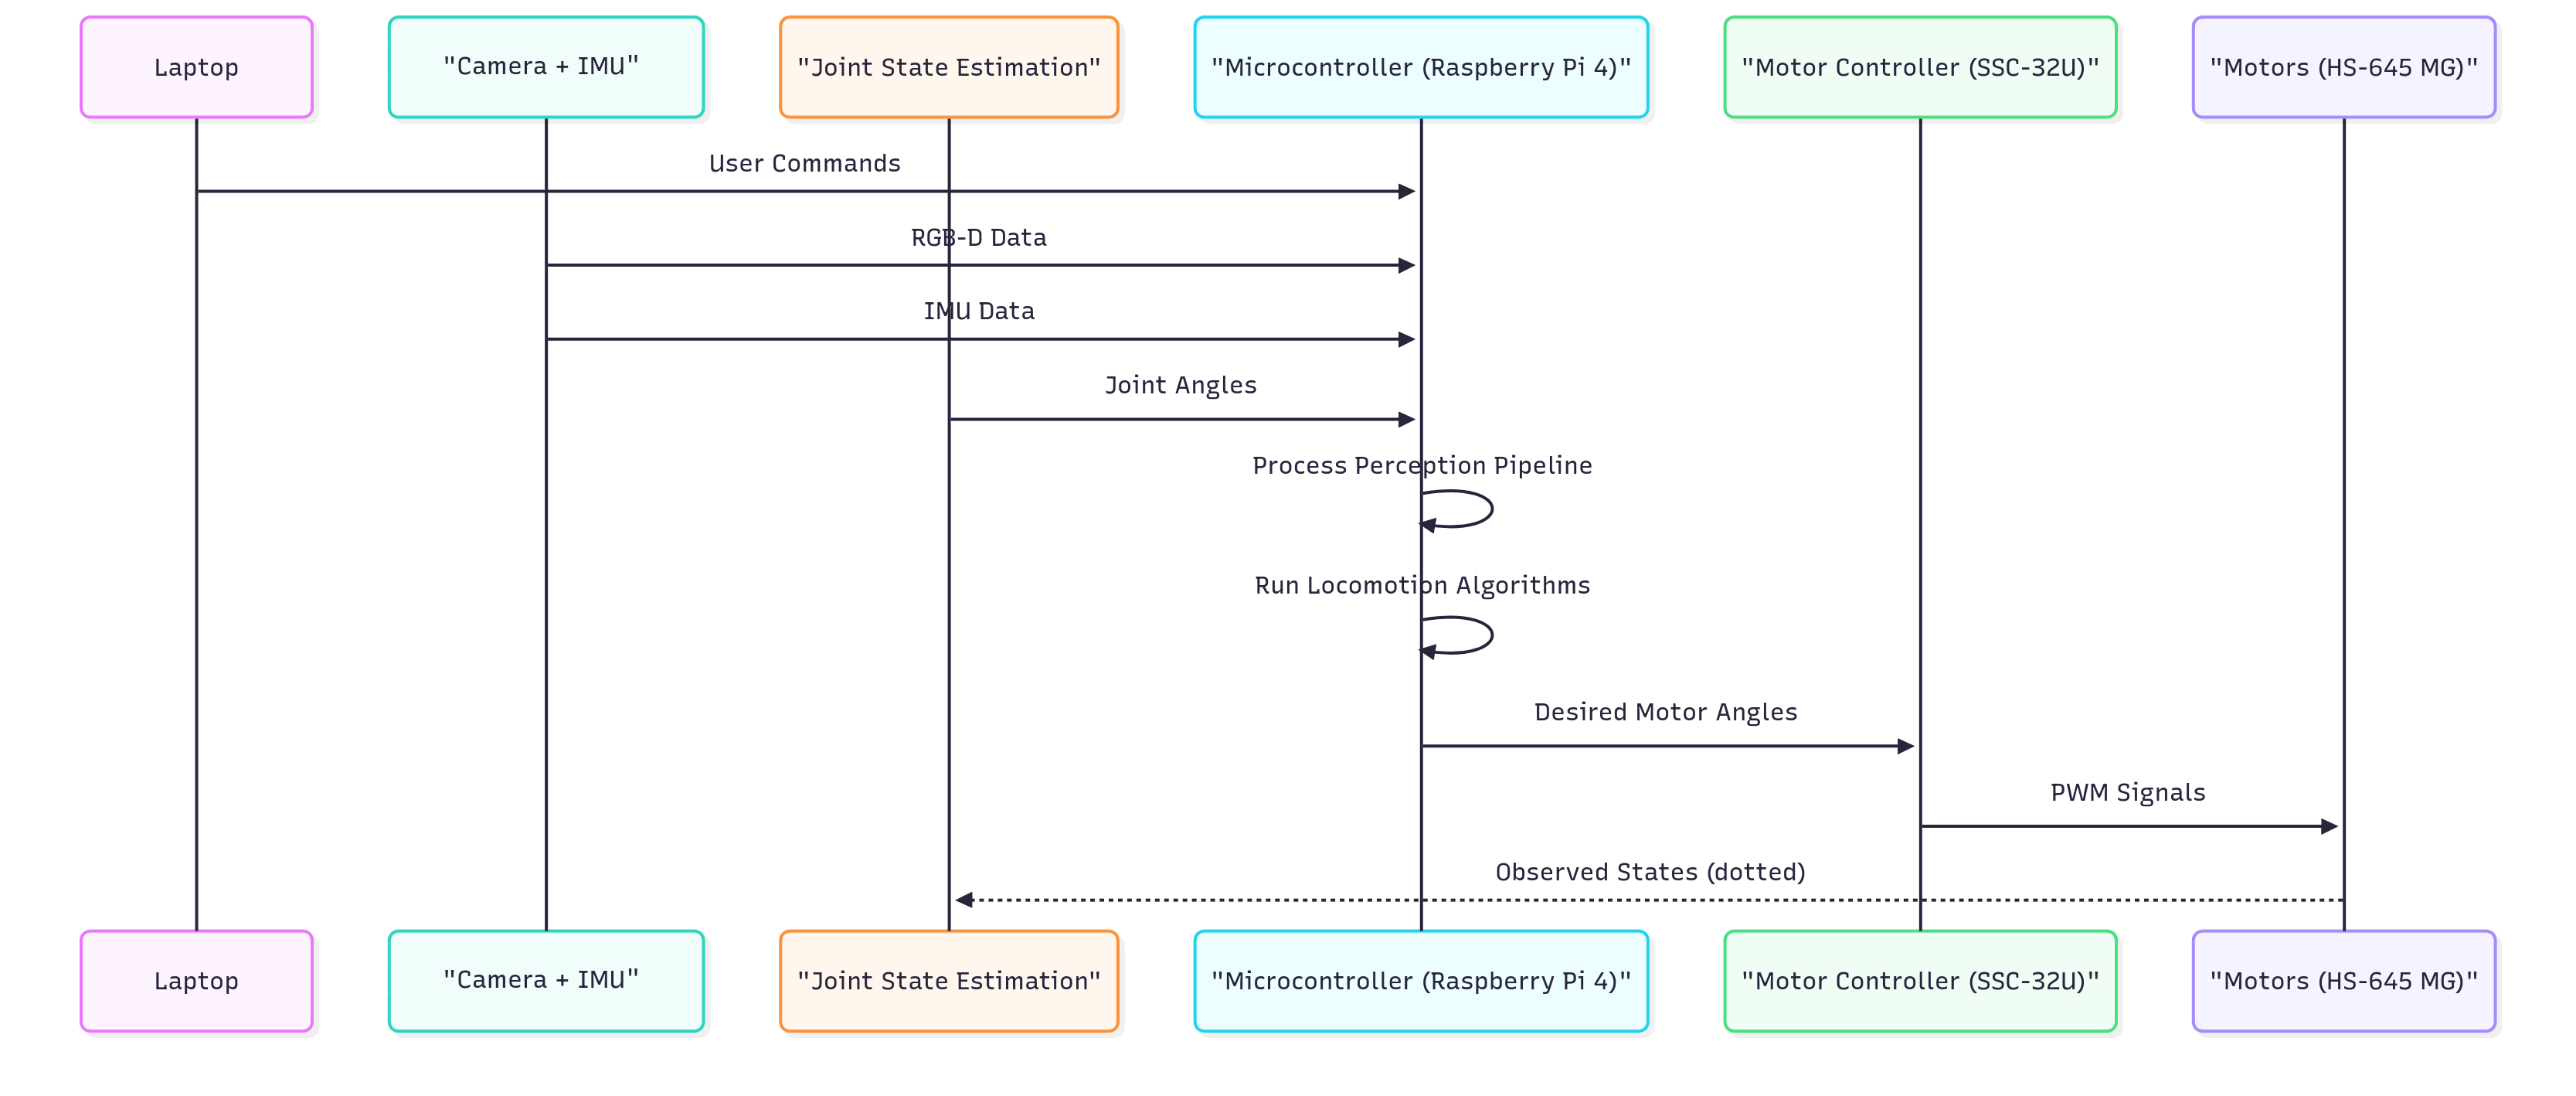
\includegraphics[width=1.0\textwidth]{hardware.png}
    \caption{Sequence Diagram for the Hardware Pipeline, showing the flow of data and commands between physical components.}
    \label{fig:hardware_diagram}
\end{figure}

\section{Technical Details}

Here, we discuss algorithms. Further information is provided in the Robot Technical Document.

The Trajectory Planning Algorithm handles movement. Using Model Predictive Control (MPC), it processes user commands and robot state, returning Center-of-Mass trajectories, leg forces, and swing trajectories. This is to traverse rough terrain.

Next, the  Map Building Algorithm is to build the map from raw RGB-D camera data and IMU readings, applying point cloud processing and odometry correction to generate a $2\text{D}$ elevation map for finding clearance. Essentially, points are classified to floor and ceiling based on their position with regards to the camera frame.

The Posture Adaptation Algorithm reads the elevation map and signed distance field to dynamically adjust the posture:

     Shorter: For low ceilings.
     
     Narrower: For thin gaps.

    Both: Stop.
Else no change from previous state.

The Environment Generation Algorithm uses random procedural generation based on user parameters aforementioned to create rough terrains for simulation.

The microcontroller converts movement commands from locomotion into final PWM signals sent directly to the motors.

